\documentclass[12pt]{article}
\usepackage[utf8]{inputenc}
\usepackage[catalan]{babel}
\usepackage{amsmath, amssymb, amsfonts}
\usepackage{geometry}
\usepackage{fancyhdr}
\usepackage{graphicx}
\usepackage{tikz}
\usetikzlibrary{matrix, calc}
\usepackage{tcolorbox}
\usepackage[colorlinks=true, linkcolor=blue]{hyperref}
\usepackage{float}
\usepackage{enumitem}

\setlength{\headheight}{15pt}

\geometry{a4paper, left=2cm, right=2cm, top=2.5cm, bottom=2.5cm}

\pagestyle{fancy}
\fancyhf{}
\fancyhead[L]{Matemàtiques 2n Batxillerat}
\fancyhead[R]{Derivades i les seves aplicacions}
\fancyfoot[L]{\href{mailto:orodri11@xtec.cat}{orodri11@xtec.cat}}
\fancyfoot[R]{\thepage}

% Colors més suaus per a llegibilitat en impressió
\newtcolorbox{concept}[1][]{colback=blue!5!white, colframe=blue!75!black, fonttitle=\bfseries, title=Concepte, #1}
\newtcolorbox{exemple}[1][]{colback=green!5!white, colframe=green!75!black, fonttitle=\bfseries, title=Exemple, #1}
\newtcolorbox{exercici}[1][]{colback=yellow!10!white, colframe=yellow!75!black, fonttitle=\bfseries, title=Exercici, #1}
\newtcolorbox{solucio}[1][]{colback=orange!5!white, colframe=orange!75!black, fonttitle=\bfseries, title=Solució, #1}

\begin{document}

\begin{titlepage}
    \centering
    \vspace*{1cm}
    {\Huge \textbf{Càlcul Diferencial: \\ Les Derivades i les seves aplicacions} \par}
    \vspace{0.5cm}
    {\Large Matemàtiques 2n Batxillerat \par}
    \vspace{1.5cm}
    % Substituir per la imatge real
    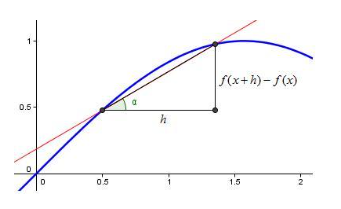
\includegraphics[width=0.5\textwidth]{derivades.png} 
    \vspace{1.5cm}
    \tableofcontents
\end{titlepage}

\newpage

\section{Repàs al concepte de límit i continuïtat}

% ---------------------------------------------------------
% SUBSECCIÓ: LÍMITS
% ---------------------------------------------------------
\subsection{El concepte de Límit}

\begin{concept}
\textbf{Límits Laterals}\\
Donada una funció $f(x)$, i un punt fix $x=a$:
\begin{itemize}
    \item \textbf{Límit per l'esquerra:} Direm que la funció tendeix a $b$ quan $x$ s'apropa a $a$ per l'esquerra, i escriurem:
    \[ \lim_{x\to a^-} f(x) = b \]
    Això succeeix quan la gràfica de la funció tendeix a $b$ a mesura que $x$ s'apropa més i més a $a$ amb valors menors que $a$ (és a dir, sempre a l'esquerra de $a$).
    
    \item \textbf{Límit per la dreta:} Direm que la funció tendeix a $b$ quan $x$ s'apropa a $a$ per la dreta, i escriurem:
    \[ \lim_{x\to a^+} f(x) = b \]
    Això succeeix quan la gràfica de la funció tendeix a $b$ a mesura que $x$ s'apropa més i més a $a$ amb valors majors que $a$ (és a dir, sempre a la dreta de $a$).
\end{itemize}

\textbf{Definició pràctica de límit}\\
Donada una funció $f(x)$ i un punt fix $x=a$, direm que la funció tendeix a $b$ quan $x$ s'apropa a $a$, i escriurem:
\[ \lim_{x\to a} f(x) = b \]
Això passa quan existeixen els dos límits laterals i coincideixen, és a dir, quan la gràfica de la funció tendeix a $b$ a mesura que $x$ s'apropa més i més a $a$, tant per la dreta com per l'esquerra:
\[ \lim_{x\to a^-} f(x) = \lim_{x\to a^+} f(x) = b \implies \lim_{x\to a} f(x) = b \]

\textbf{Nota important:}\\
En el concepte de límit no apareix enlloc el valor $f(a)$. Tant és quant valgui $f(a)$. Fins i tot, la funció pot no estar definida en $x=a$.
\end{concept}

\begin{figure}[h]
    \centering
    % Substituir per la imatge real
    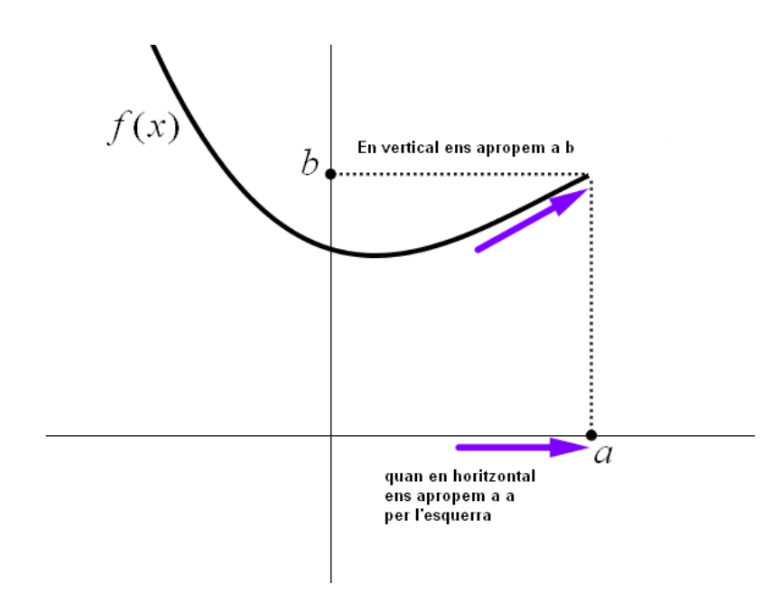
\includegraphics[width=0.7\textwidth]{esquerra.png}
    \caption{Aproximació al punt $x=a$ per l'esquerra i la seva repercussió vertical cap a $b$.}
\end{figure}

\begin{concept}
\textbf{Exemple}\\
Donada la funció $f(x) = \frac{x}{x}$, aquesta no està definida en $x=0$; tanmateix:
\[ \lim_{x\to 0^+} f(x) = 1 \quad \text{i} \quad \lim_{x\to 0^-} f(x) = 1 \]
Com que existeixen els límits laterals i coincideixen, tenim que:
\[ \lim_{x\to 0} f(x) = 1 \]
\end{concept}

\begin{concept}
\textbf{Límits infinits i comportament en l'infinit}\\
El concepte de límit es pot ampliar si $a$ o $b$ prenen els símbols $+\infty$ o $-\infty$, sempre que tinguem clar que $\infty$ no és un nombre, sinó una tendència.

\textbf{Límits infinits:}
\begin{itemize}
    \item $\lim_{x\to a^+} f(x) = +\infty$ equival a la frase ``la funció es fa més i més gran en positiu a mesura que $x$ s'apropa més i més a $a$ per la dreta''.
    \item $\lim_{x\to a^+} f(x) = -\infty$ equival a la frase ``la funció es fa més i més gran en negatiu a mesura que $x$ s'apropa més i més a $a$ per la dreta''. \textit{(S'aplica la mateixa lògica per l'esquerra)}.
\end{itemize}

\textbf{Comportament en l'infinit:}
\begin{itemize}
    \item $\lim_{x\to +\infty} f(x) = b$ equival a la frase ``la funció s'apropa a $b$ quan la $x$ es fa més i més gran en positiu''.
    \item $\lim_{x\to -\infty} f(x) = b$ equival a la frase ``la funció s'apropa a $b$ quan la $x$ es fa més i més gran en negatiu''.
\end{itemize}
\end{concept}

\begin{figure}[h]
    \centering
    % Substituir per la imatge real
    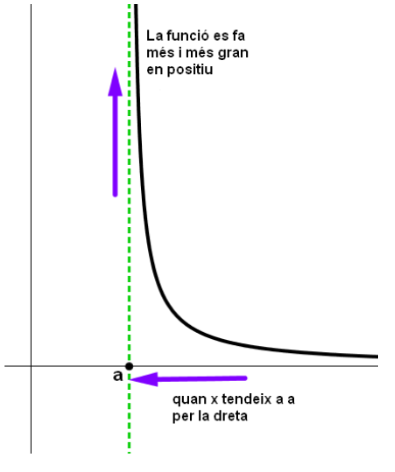
\includegraphics[width=0.4\textwidth]{limitinfinit.png}
    \caption{Quan $x=a$ per l'esquerra i la funció tendeix a infinit.}
\end{figure}

\begin{figure}[h]
    \centering
    % Substituir per la imatge real
    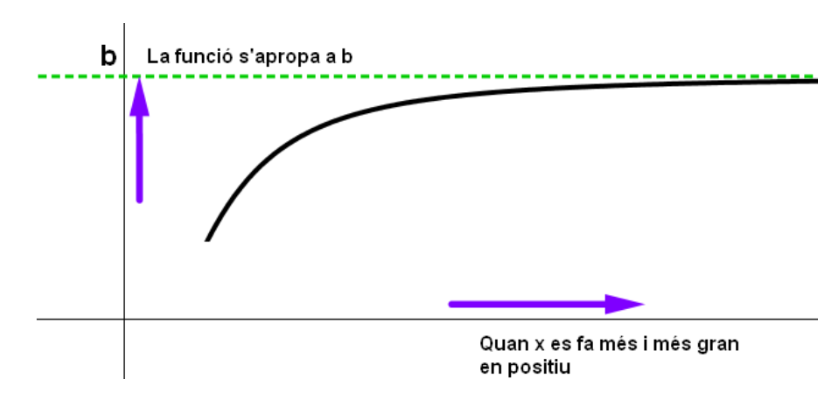
\includegraphics[width=0.7\textwidth]{limitainfinit.png}
    \caption{Quan $x$ es fa molt i molt gran la funció tendeix a $b$.}
\end{figure}

% --- NOU: Propietats algebraiques dels límits ---
\begin{concept}
\textbf{Propietats algebraiques dels límits}\\
Si $\lim_{x\to a} f(x) = L$ i $\lim_{x\to a} g(x) = M$ (amb $L,M$ finits), aleshores:
\begin{align*}
    \lim_{x\to a} (f(x) \pm g(x)) &= L \pm M, \\
    \lim_{x\to a} (k \cdot f(x)) &= k \cdot L \quad \text{(amb $k$ constant)}, \\
    \lim_{x\to a} (f(x) \cdot g(x)) &= L \cdot M, \\
    \lim_{x\to a} \frac{f(x)}{g(x)} &= \frac{L}{M} \quad \text{si } M \neq 0.
\end{align*}
Aquestes propietats també són vàlides per a límits laterals i per a límits en l'infinit, sempre que les expressions tinguin sentit.
\end{concept}

\begin{concept}
\textbf{Indeterminacions}\\
En calcular límits, en el moment de substituir la variable $x$ per la seva tendència, sovint ens trobarem amb expressions matemàtiques que no proporcionen un resultat directe o evident. Aquestes expressions s'anomenen \textbf{indeterminacions}. 

L'aparició d'una indeterminació no significa que el límit no existeixi, sinó que cal utilitzar tècniques algebraiques (com factoritzar, simplificar, multiplicar pel conjugat, etc.) per resoldre'l i trobar-ne el valor real. Les principals indeterminacions són:
\[ \infty-\infty, \quad \infty\cdot 0, \quad \frac{0}{0}, \quad \frac{\infty}{\infty}, \quad 1^\infty, \quad \infty^0, \quad 0^0 \]
\end{concept}

\begin{exemple}
\textbf{Càlcul d'un límit directe i una indeterminació}\\
Si avaluem el límit de $f(x) = x^2 + 2$ quan $x \to 1$, simplement substituïm:
\[ \lim_{x\to 1} (x^2 + 2) = 1^2 + 2 = 3 \]
En canvi, si tenim $\lim_{x\to 2} \frac{x^2 - 4}{x - 2}$, obtenim la indeterminació $0/0$. Podem resoldre-la factoritzant el numerador:
\[ \lim_{x\to 2} \frac{(x-2)(x+2)}{x-2} = \lim_{x\to 2} (x+2) = 4 \]
\end{exemple}

% --- EXERCICIS AMPLIATS ---
\begin{exercici}
Calcula els següents límits:
\begin{enumerate}
    \item $\lim_{x\to 3} \frac{x^2 - 9}{x - 3}$
    \item $\lim_{x\to \infty} \frac{2x^2 + 3x}{x^2 - 1}$
    \item $\lim_{x\to \infty} \left(\sqrt{x^2+x} - x\right)$ \quad (Ind. $\infty-\infty$)
    \item $\lim_{x\to 0} \frac{\sin x}{x}$ \quad (Utilitza la regla de l'Hôpital si la coneixes, o pensa en la definició de derivada del sinus)
    \item $\lim_{x\to \infty} \left(1+\frac{1}{x}\right)^x$ \quad (Ind. $1^\infty$)
\end{enumerate}
\end{exercici}


% ---------------------------------------------------------
% SUBSECCIÓ: CONTINUÏTAT
% ---------------------------------------------------------
\subsection{El concepte de Continuïtat}

\begin{concept}
\textbf{Interpretació visual i Definició Formal}\\
Visualment, una funció té una discontinuïtat en un punt quan la seva gràfica està ``trencada''; seguint el símil d'una mànega d'aigua, seria un punt on hi ha una fuita. Si una funció no té discontinuïtats, direm que és contínua.

Formalment, una funció $f(x)$ és contínua en $x=a$ si compleix:
\[ \lim_{x\to a^-} f(x) = \lim_{x\to a^+} f(x) = f(a) \]

\textbf{Continuïtat en un interval}\\
Direm que $f$ és contínua en un interval obert $(a,b)$ si ho és en tots els punts d'aquest interval. Si l'interval és tancat $[a,b]$, cal exigir continuïtat en els extrems per un sol lateral: per l'esquerra a $b$ i per la dreta a $a$.

\textbf{Operacions amb funcions contínues}\\
Qualsevol \textbf{funció polinòmica} és contínua en tota la recta real ($\mathbb{R}$). Les funcions racionals són contínues en el seu domini (excepte on s'anul·la el denominador). A més, si tenim dues funcions que són contínues en un cert punt $a$, la seva suma, resta, producte, composició i quocient (si el denominador no és zero) també seran funcions contínues en $a$.
\end{concept}

\begin{figure}[h]
    \centering
    % Substituir per la imatge real
    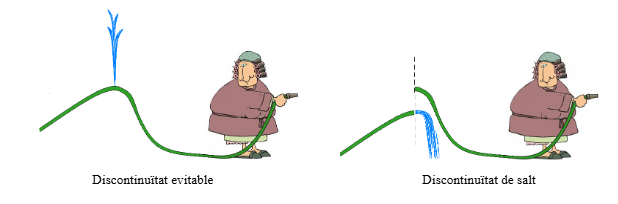
\includegraphics[width=0.6\textwidth]{contvsdiscont.png}
    \caption{A l'esquerra funció contínua, a la dreta funció amb discontinuïtat.}
\end{figure}

% ---------------------------------------------------------
% SUBSECCIÓ: TIPUS DE DISCONTINUÏTATS
% ---------------------------------------------------------
\subsection{Tipus de discontinuïtats notables}

\begin{concept}
Quan les condicions de continuïtat fallen en un punt, ens trobem davant d'una discontinuïtat. Es classifiquen en:
\begin{itemize}
    \item \textbf{Discontinuïtat evitable:} Els límits laterals coincideixen ($L$), però la funció no hi està definida o $f(a) \neq L$. (Petit forat a la gràfica).
    \item \textbf{Discontinuïtat inevitable de salt finit:} Els límits laterals existeixen però són diferents entre ells. (Salt en la gràfica).
    \item \textbf{Discontinuïtat inevitable de salt infinit (Asímptota vertical):} Almenys un dels límits laterals tendeix cap a l'infinit ($\pm \infty$).
\end{itemize}

Per a les \textbf{funcions a trossos}, l'estratègia és centrar l'atenció en els punts frontera i verificar-hi que els límits per l'esquerra, per la dreta i la imatge del punt coincideixin.
\end{concept}

% --- TAULA RESUM (VERSIÓ DEFINITIVA) ---
\begin{concept}
\textbf{Resum de tipus de discontinuïtats}

\begin{center}
\small
\renewcommand{\arraystretch}{1.4}
\begin{tabular}{|c|p{4.2cm}|p{4.2cm}|}
\hline
\textbf{Tipus} & \textbf{Condició} & \textbf{Exemple} \\
\hline
\textbf{Evitable} & 
$\displaystyle\lim_{x\to a^-}f=\lim_{x\to a^+}f=L$ però $f(a)$ no existeix o $f(a)\neq L$ &
$f(x)=\dfrac{x^2-1}{x-1}$ (en $x=1$ no definida o redefinida) \\[0.3cm]
\hline
\textbf{Salt finit} & 
$\displaystyle\lim_{x\to a^-}f=L_1$, $\displaystyle\lim_{x\to a^+}f=L_2$ amb $L_1\neq L_2$ (finits) &
$f(x)=\begin{cases}x & x\leq 0 \\ x+1 & x>0 \end{cases}$ \\[0.3cm]
\hline
\textbf{Salt infinit} & 
Almenys un dels límits laterals és $\pm\infty$ &
$f(x)=\dfrac{1}{x}$ en $x=0$ \\[0.3cm]
\hline
\end{tabular}
\normalsize
\end{center}

\textbf{Observacions:}
\begin{itemize}
    \item En la discontinuïtat evitable, el límit existeix però no coincideix amb el valor de la funció (o la funció no està definida en el punt). Es pot "evitar" redefinint la funció en el punt.
    \item En la discontinuïtat de salt finit, la funció "salta" d'un valor a un altre; els límits laterals són finits però diferents.
    \item En la discontinuïtat de salt infinit, la funció tendeix a $\pm\infty$, cosa que produeix una asímptota vertical.
\end{itemize}
\end{concept}

% --- GRÀFICS AMB TIKZ (disposició horitzontal) ---
\subsection*{Representació gràfica}

\begin{center}
\begin{tikzpicture}[scale=0.7]

% ---- DISCONTINUÏTAT EVITABLE (esquerra) ----
\begin{scope}[xshift=-7cm, yshift=0cm]
    \draw[->] (-3,0) -- (3,0);
    \draw[->] (0,-0.5) -- (0,3.5);
    % Paràbola
    \draw[domain=-3:3, smooth, variable=\x, blue, thick] 
        plot ({\x}, {0.4*(\x)^2 + 0.8});
    % Forat
    \draw[fill=white, draw=red, thick] (1.2,1.376) circle (4pt);
    % Punt redefinit
    \draw[fill=red, draw=red, thick] (1.2,2.8) circle (4pt);
    \node[below] at (1.2,-0.2) {$a$};
    \node[red, left] at (0.8,2.8) {$f(a)$};
    \node[red, right] at (1.6,1.376) {$L$};
    \node[blue, above] at (0,3.3) {\textbf{Evitable}};
\end{scope}

% ---- DISCONTINUÏTAT DE SALT FINIT (centre) ----
\begin{scope}[xshift=0cm, yshift=0cm]
    \draw[->] (-3,0) -- (3,0);
    \draw[->] (0,-0.5) -- (0,3.5);
    % Branca esquerra
    \draw[domain=-3:0, smooth, variable=\x, blue, thick] 
        plot ({\x}, {0.4*\x + 1.2});
    % Branca dreta
    \draw[domain=0:3, smooth, variable=\x, blue, thick] 
        plot ({\x}, {0.4*\x + 2.8});
    \draw[fill=blue, draw=blue, thick] (0,1.2) circle (4pt);
    \draw[fill=white, draw=blue, thick] (0,2.8) circle (4pt);
    \node[below] at (0,-0.2) {$a$};
    \node[blue, left] at (-0.5,1.2) {$L_1$};
    \node[blue, right] at (0.5,2.8) {$L_2$};
    \node[blue, above] at (0,3.3) {\textbf{Salt finit}};
\end{scope}

% ---- DISCONTINUÏTAT DE SALT INFINIT (dreta) ----
\begin{scope}[xshift=7cm, yshift=0cm]
    \draw[->] (-3,0) -- (3,0);
    \draw[->] (0,-3.5) -- (0,3.5);
    % Branca esquerra
    \draw[domain=-3:-0.25, smooth, variable=\x, blue, thick] 
        plot ({\x}, {1.2/\x});
    % Branca dreta
    \draw[domain=0.25:3, smooth, variable=\x, blue, thick] 
        plot ({\x}, {1.2/\x});
    \draw[dashed, red, thick] (0,-3.5) -- (0,3.5);
    \node[below] at (0,-0.2) {$a$};
    \node[red, rotate=90] at (-0.6,0) {Asímptota vertical};
    \node[blue, above] at (0,3.3) {\textbf{Salt infinit}};
\end{scope}

\end{tikzpicture}

\vspace{0.3cm}
\textit{Representació gràfica dels tres tipus de discontinuïtats.}
\end{center}

\begin{exemple}
\textbf{Classificació de discontinuïtats}\\
Classifica la discontinuïtat de les següents funcions en els punts indicats:
\begin{enumerate}
    \item $f(x)=\dfrac{x^2-4}{x-2}$ en $x=2$
    \item $f(x)=\begin{cases} x+1 & x<0 \\ x-1 & x\ge 0 \end{cases}$ en $x=0$
    \item $f(x)=\dfrac{1}{(x-1)^2}$ en $x=1$
\end{enumerate}
\textbf{Solucions:}
\begin{enumerate}
    \item $\lim_{x\to 2} f(x)=4$ però $f(2)$ no existeix $\Rightarrow$ \textbf{evitable}.
    \item $\lim_{x\to 0^-} f(x)=1$, $\lim_{x\to 0^+} f(x)=-1$ $\Rightarrow$ \textbf{salt finit}.
    \item $\lim_{x\to 1} f(x)=+\infty$ $\Rightarrow$ \textbf{salt infinit}.
\end{enumerate}
\end{exemple}

% --- EXEMPLE IL·LUSTRATIU ---
\begin{exemple}
\textbf{Exemple de discontinuïtat evitable}\\
Sigui 
\[
f(x)=\frac{x^2-1}{x-1}
\]
Aquesta funció no està definida en $x=1$. Tanmateix:
\[
\lim_{x\to 1} \frac{x^2-1}{x-1} = \lim_{x\to 1} \frac{(x-1)(x+1)}{x-1} = \lim_{x\to 1} (x+1)=2
\]
Per tant, la discontinuïtat és \textit{evitable}: bastaria definir $f(1)=2$ perquè la funció sigui contínua en $x=1$.
\end{exemple}

% Exemple previ a l'exercici: funció a trossos amb discontinuïtat de salt
\begin{exemple}
\textbf{Estudi d'una funció a trossos amb salt finit}\\
Sigui 
\[
f(x) = \begin{cases} 
      x+1 & \text{si } x < 2, \\
      x^2-2 & \text{si } x \geq 2.
   \end{cases}
\]
Estudiem la continuïtat en $x=2$:
\begin{itemize}
    \item Límit per l'esquerra: $\lim_{x\to 2^-} (x+1) = 3$.
    \item Límit per la dreta: $\lim_{x\to 2^+} (x^2-2) = 4-2=2$.
    \item Imatge: $f(2)=2^2-2=2$ (pertany al segon tram).
\end{itemize}
Com que els límits laterals no coincideixen ($3\neq 2$), hi ha una discontinuïtat de salt finit en $x=2$.
\end{exemple}

\begin{exercici}
Estudia la continuïtat de la següent funció definida a trossos i indica el tipus de discontinuïtat si n'hi ha:
\[
f(x) = \begin{cases} 
      x^2 + 1 & \text{si } x \leq 1, \\
      3x - 1 & \text{si } x > 1.
   \end{cases}
\]
\end{exercici}

% --- NOU: Segon exercici de continuïtat per practicar ---
\begin{exercici}
Donada la funció
\[
g(x) = \begin{cases}
      \dfrac{x^2-4}{x-2} & \text{si } x \neq 2, \\
      5 & \text{si } x = 2,
   \end{cases}
\]
determina si és contínua en $x=2$. En cas contrari, classifica la discontinuïtat.
\end{exercici}

% ---------------------------------------------------------
% SUBSECCIÓ: TEOREMA DE BOLZANO
% ---------------------------------------------------------
\subsection{Teorema de Bolzano}

\begin{concept}
Aquest teorema és una de les aplicacions més útils de la continuïtat, ens assegura que una gràfica creua l'eix de les abscisses sense necessitat de dibuixar-la ni resoldre l'equació de forma exacta.

\textbf{Enunciat:}\\
Si una funció $f(x)$ és contínua en un interval tancat $[a,b]$ i els signes en els extrems d'aquest interval són oposats ($f(a) \cdot f(b) < 0$), aleshores existeix com a mínim un punt $c \in (a,b)$ tal que la funció s'anul·la ($f(c)=0$).

\textbf{Observacions importants:}
\begin{itemize}
    \item El teorema \textbf{no proporciona} el valor de $c$, només garanteix la seva existència.
    \item El resultat permet localitzar intervals que contenen solucions d'equacions, i sovint s'utilitza juntament amb mètodes numèrics per aproximar-les.
    \item La condició de continuïtat és essencial; si la funció té un salt, pot no creuar l'eix encara que els extrems tinguin signes oposats.
\end{itemize}
\end{concept}

\begin{figure}[h]
    \centering
    % Substituir per la imatge real
    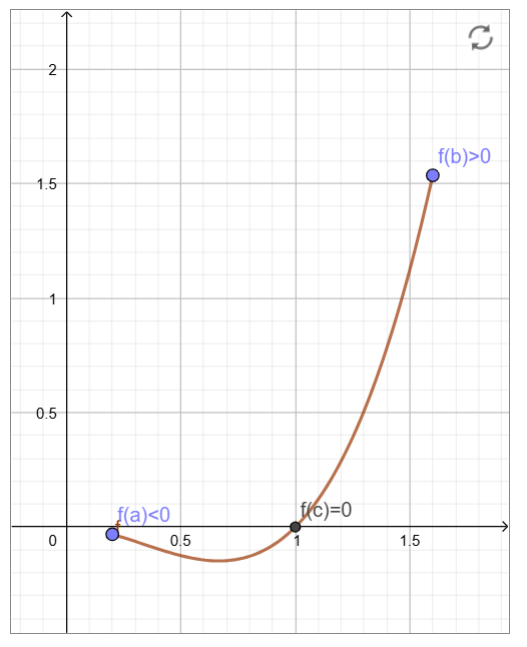
\includegraphics[width=0.6\textwidth]{Bolzano.png}
    \caption{Interpretació geomètrica de Bolzano: en passar contínuament d'una alçada negativa a una positiva, obligatòriament creuem l'eix X ($y=0$).}
\end{figure}

\begin{exemple}
\textbf{Aplicació del Teorema de Bolzano}\\
Demostrem que l'equació $x^3 + x - 1 = 0$ té almenys una solució real entre $0$ i $1$.\\
1. Definim la funció $f(x) = x^3 + x - 1$, que és contínua a $\mathbb{R}$ per ser polinòmica.\\
2. Avaluem als extrems de l'interval $[0, 1]$: 
   \begin{itemize}
       \item $f(0) = 0^3 + 0 - 1 = -1$ (Negatiu)
       \item $f(1) = 1^3 + 1 - 1 = 1$ (Positiu)
   \end{itemize}
3. Com que hi ha canvi de signe, el Teorema de Bolzano garanteix que existeix $c \in (0,1)$ on $f(c) = 0$. Per tant, l'equació té solució en aquest interval.
\end{exemple}

\begin{exercici}
Demostra que l'equació $2^x = 4 - x$ té almenys una solució en l'interval $(1,2)$.
\end{exercici}

% ---------------------------------------------------------
% ENLLAÇ AMB DERIVADES (més ampliat)
% ---------------------------------------------------------
\subsection{Per què tot aquest repàs?}

Els conceptes de límit i continuïtat són la base sobre la qual es construeix el càlcul diferencial. La \textbf{derivada} d'una funció en un punt es defineix com un límit:
\[
f'(a) = \lim_{h\to 0} \frac{f(a+h)-f(a)}{h}
\]
Aquest quocient incremental només té sentit si el límit existeix (és a dir, si els límits laterals coincideixen). Per tant, entendre bé els límits i la continuïtat és imprescindible per comprendre el significat de la derivada, la seva interpretació geomètrica (pendent de la recta tangent) i les seves aplicacions (optimització, càlcul de taxes de variació, etc.). En les properes seccions, aprofundirem en aquesta eina fonamental.



% ---------------------------------------------------------
% NOU CAPÍTOL: DERIVADES
% ---------------------------------------------------------
\section{La Derivada}

\subsection{Derivada d'una funció en un punt}

\begin{concept}
\textbf{Definició de derivada en un punt}\\
Donada una funció real $f$ i un punt d'abscissa $x=a$ (amb $a \in D_f$), considerem el límit següent:
\[
\lim_{h\to 0} \frac{f(a+h)-f(a)}{h}
\]
Si aquest límit existeix, s'anomena \textbf{derivada de la funció $f$ en $x=a$}, i s'escriu $f'(a)$:
\[
\boxed{f'(a)=\lim_{h\to 0} \frac{f(a+h)-f(a)}{h}}
\]

\textbf{Expressió alternativa}\\
Si fem el canvi de variable $a+h = x$, aleshores $h = x-a$ i quan $h\to 0$ tenim $x\to a$. Per tant:
\[
\boxed{f'(a)=\lim_{x\to a} \frac{f(x)-f(a)}{x-a}}
\]
\end{concept}

\begin{exemple}
\textbf{Exemple 1}\\
Donada $f(x)=7x-3$, calculem $f'(a)$ per a qualsevol $a\in\mathbb{R}$.
\[
f'(a)=\lim_{x\to a} \frac{f(x)-f(a)}{x-a}
      =\lim_{x\to a} \frac{7x-3-(7a-3)}{x-a}
      =\lim_{x\to a} \frac{7(x-a)}{x-a}=7
\]
Per tant, $f'(a)=7$ per a tot $a\in\mathbb{R}$.
\end{exemple}

\begin{exemple}
\textbf{Exemple 2}\\
Esbrineu si existeix la derivada en els punts $x=0$, $x=2$ i $x=-2$ de la funció a trossos:
\[
f(x)=
\begin{cases}
2x+1 & \text{si } x\le 0 \\
x-1 & \text{si } x>0
\end{cases}
\]
Per calcular la derivada en aquests punts, hem de calcular els límits que defineixen $f'(0)$, $f'(2)$ i $f'(-2)$.

\textbf{Per a $x=0$:}
\[
f'(0)=\lim_{x\to 0} \frac{f(x)-f(0)}{x-0}
\]
Calculem els límits laterals:
\[
\lim_{x\to 0^+} \frac{f(x)-f(0)}{x}
= \lim_{x\to 0^+} \frac{x-1-1}{x}
= \lim_{x\to 0^+} \frac{x-2}{x} = -\infty
\]
\[
\lim_{x\to 0^-} \frac{f(x)-f(0)}{x}
= \lim_{x\to 0^-} \frac{2x+1-1}{x}
= \lim_{x\to 0^-} \frac{2x}{x} = 2
\]
Com que els límits laterals no coincideixen, el límit no existeix. Per tant, $f'(0)$ no existeix.

\textbf{Per a $x=2$:}
\[
f'(2)=\lim_{x\to 2} \frac{f(x)-f(2)}{x-2}
      =\lim_{x\to 2} \frac{x-1-1}{x-2}
      =\lim_{x\to 2} \frac{x-2}{x-2}=1
\]

\textbf{Per a $x=-2$:}
\[
f'(-2)=\lim_{x\to -2} \frac{f(x)-f(-2)}{x+2}
       =\lim_{x\to -2} \frac{2x+1-(-3)}{x+2}
       =\lim_{x\to -2} \frac{2x+4}{x+2}
       =\lim_{x\to -2} \frac{2(x+2)}{x+2}=2
\]
\end{exemple}


\subsection{Interpretació geomètrica de la derivada}

Per entendre el significat geomètric de la derivada \href{https://mdosil.github.io/mates2batcientific/temes/derivades/}{fixeu-vos amb el gràfic següent}.

\begin{figure}[h]
    \centering
    % Substituir per la imatge real
    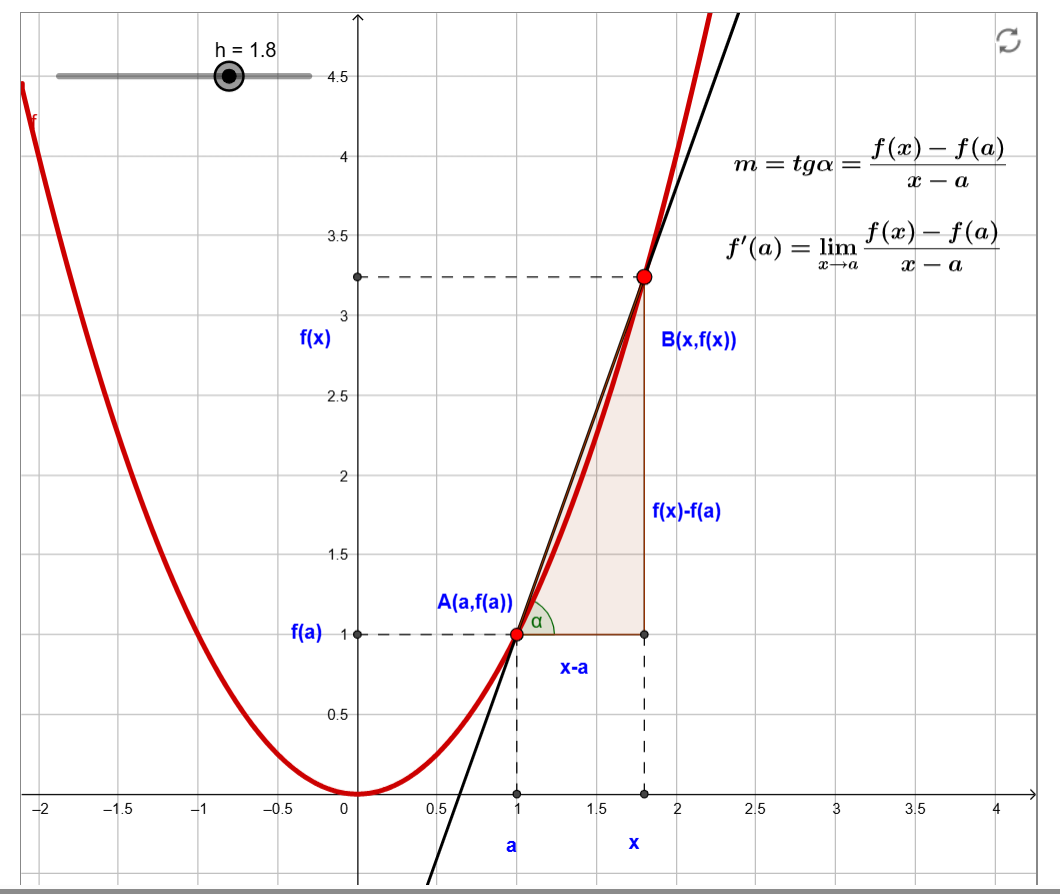
\includegraphics[width=0.45\textwidth]{conceptederivada.png}
    \caption{La recta secant tendeix a ser la recta tangent a la funció quan $x$ s'aproxima a $a$.}
\end{figure}

\begin{concept}
\textbf{De la secant a la tangent}\\
Considerem la gràfica d'una funció $f$. Prenem dos punts:
\begin{itemize}
    \item $A=(a,f(a))$ (punt fix),
    \item $B=(x,f(x))$ (punt variable).
\end{itemize}
La recta que passa per $A$ i $B$ s'anomena \textbf{recta secant}. El seu pendent és:
\[
m_{\text{secant}}=\frac{f(x)-f(a)}{x-a}
\]
Aquesta expressió també es coneix com a \textbf{taxa de variació mitjana (TVM)} entre $x$ i $a$.

Si anem acostant el punt $B$ al punt $A$ (és a dir, fem $x\to a$), la recta secant es va aproximant a una recta límit que anomenem \textbf{recta tangent} a la corba en $x=a$. El pendent d'aquesta recta tangent és:
\[
m_{\text{tangent}}=\lim_{x\to a} \frac{f(x)-f(a)}{x-a}=f'(a)
\]

Per tant:
\[
\boxed{f'(a) \text{ és el pendent de la recta tangent a la gràfica de } f \text{ en el punt } x=a}
\]

\textbf{Relació amb el creixement:}
\begin{itemize}
    \item Si $f'(a)>0$, la funció és creixent en $a$ (pendent positiu).
    \item Si $f'(a)<0$, la funció és decreixent en $a$ (pendent negatiu).
    \item Si $f'(a)=0$, la recta tangent és horitzontal.
\end{itemize}
\end{concept}


\subsection{Recta tangent a una corba en un punt}

\begin{concept}
\textbf{Equació de la recta tangent}\\
Donada una funció $f$ derivable en $x=a$, la recta tangent a la seva gràfica en el punt $(a,f(a))$ és la recta que:
\begin{itemize}
    \item conté el punt $(a,f(a))$,
    \item té pendent $m=f'(a)$.
\end{itemize}
Per tant, la seva equació és:
\[
\boxed{y-f(a)=f'(a)\,(x-a)}
\]
\end{concept}

\begin{exemple}
\textbf{Exemple 3}\\
Trobeu l'equació de la recta tangent a la funció $f(x)=3x^2-5x+2$ en el punt d'abscissa $x=1$.

El punt de tangència és $(1,f(1))=(1,0)$. Calculem la derivada en $x=1$:
\[
f'(1)=\lim_{x\to 1} \frac{f(x)-f(1)}{x-1}
      =\lim_{x\to 1} \frac{3x^2-5x+2-0}{x-1}
      =\lim_{x\to 1} \frac{(3x-2)(x-1)}{x-1}
      =\lim_{x\to 1} (3x-2)=1
\]
Per tant, l'equació de la recta tangent és:
\[
y-0=1(x-1) \quad\Longrightarrow\quad \boxed{y=x-1}
\]
\end{exemple}


\subsection{Relació entre la derivada i la continuïtat (demostració)}

\begin{concept}
\textbf{Teorema}\\
Si una funció $f$ és derivable en $x=a$, aleshores $f$ és contínua en $x=a$.

És important remarcar que \textbf{el recíproc no és cert}: una funció pot ser contínua en un punt però no derivable (per exemple, $f(x)=|x|$ en $x=0$).

\textbf{Contrarecíproc (equivalent):}\\
Si una funció no és contínua en $x=a$, aleshores no és derivable en $x=a$.
\end{concept}

\begin{concept}
\textbf{Demostració del teorema}\\
Suposem que $f$ és derivable en $x=a$. Això vol dir que existeix:
\[
f'(a)=\lim_{x\to a} \frac{f(x)-f(a)}{x-a}
\]
Volem veure que $\lim_{x\to a} f(x)=f(a)$. Escrivim:
\[
f(x)-f(a)=\frac{f(x)-f(a)}{x-a}\cdot (x-a)
\]
Prenent límits quan $x\to a$:
\[
\lim_{x\to a} (f(x)-f(a))
=
\lim_{x\to a} \frac{f(x)-f(a)}{x-a}
\cdot
\lim_{x\to a} (x-a)
=
f'(a)\cdot 0 = 0
\]
Per tant:
\[
\lim_{x\to a} f(x)-f(a)=0
\quad\Longrightarrow\quad
\lim_{x\to a} f(x)=f(a)
\]
I això és precisament la definició de continuïtat en $x=a$. $\square$
\end{concept}

\begin{exemple}
\textbf{Exemple 4}\\
Estudia la derivabilitat de la funció a trossos:
\[
f(x)=
\begin{cases}
2x^2-3x-1 & \text{si } x\le -1 \\
4x+1 & \text{si } x>-1
\end{cases}
\]

\textbf{Solució:}
El punt de canvi és $x=-1$. Calculem els límits laterals del quocient incremental:

Per l'esquerra ($x\le -1$):
\begin{align*}
\lim_{x\to -1^-} \frac{f(x)-f(-1)}{x+1} 
&= \lim_{x\to -1^-} \frac{(2x^2-3x-1) - (2+3-1)}{x+1} \\
&= \lim_{x\to -1^-} \frac{2x^2-3x-1 - 4}{x+1} \\
&= \lim_{x\to -1^-} \frac{2x^2-3x-5}{x+1}
\end{align*}
Factoritzem el numerador: $2x^2-3x-5 = (x+1)(2x-5)$. Per tant:
\[
\lim_{x\to -1^-} \frac{(x+1)(2x-5)}{x+1}
= \lim_{x\to -1^-} (2x-5) = -7
\]

Per la dreta ($x>-1$):
\[
\lim_{x\to -1^+} \frac{f(x)-f(-1)}{x+1}
= \lim_{x\to -1^+} \frac{(4x+1)-4}{x+1}
= \lim_{x\to -1^+} \frac{4x-3}{x+1}
\]
Substituint directament: $\frac{-4-3}{0} = \frac{-7}{0} = -\infty$.

Com que els límits laterals no coincideixen (un és $-7$ i l'altre $-\infty$), la funció no és derivable en $x=-1$.
\end{exemple}


% ---------------------------------------------------------
% LA FUNCIÓ DERIVADA
% ---------------------------------------------------------
\subsection{La funció derivada}

\begin{concept}
\textbf{Definició de funció derivada}\\
Donada una funció $f$, definim la seva \textbf{funció derivada} $f'$ com aquella que a cada punt $x$ on existeix la derivada li assigna el valor $f'(x)$:
\[
\boxed{f'(x)=\lim_{h\to 0} \frac{f(x+h)-f(x)}{h}}
\]
El domini de $f'$ és el conjunt de punts on $f$ és derivable.
\end{concept}

\begin{exemple}
Calculem la funció derivada de $f(x)=x^2$:
\[
f'(x)=\lim_{h\to 0} \frac{(x+h)^2-x^2}{h}
      =\lim_{h\to 0} \frac{x^2+2xh+h^2-x^2}{h}
      =\lim_{h\to 0} \frac{2xh+h^2}{h}
      =\lim_{h\to 0} (2x+h)=2x
\]
Per tant, si $f(x)=x^2$, aleshores $f'(x)=2x$.
\end{exemple}


% ---------------------------------------------------------
% REGLES DE DERIVACIÓ
% ---------------------------------------------------------
\subsection{Regles de derivació}

\begin{concept}
\textbf{Derivada d'una constant}\\
Si $f(x)=k$ (amb $k\in\mathbb{R}$), aleshores:
\[
\boxed{f'(x)=0}
\]

\textbf{Derivada de $x$}\\
Si $f(x)=x$, aleshores:
\[
\boxed{f'(x)=1}
\]

\textbf{Derivada d'una potència}\\
Si $f(x)=x^n$ (amb $n\in\mathbb{R}$), aleshores:
\[
\boxed{f'(x)=n\,x^{n-1}}
\]

\textbf{Derivada d'una suma}\\
Si $f(x)=u(x)+v(x)$, aleshores:
\[
\boxed{f'(x)=u'(x)+v'(x)}
\]

\textbf{Derivada d'un producte per una constant}\\
Si $f(x)=k\cdot u(x)$ (amb $k\in\mathbb{R}$), aleshores:
\[
\boxed{f'(x)=k\cdot u'(x)}
\]

\textbf{Derivada d'un producte}\\
Si $f(x)=u(x)\cdot v(x)$, aleshores:
\[
\boxed{f'(x)=u'(x)\cdot v(x)+u(x)\cdot v'(x)}
\]

\textbf{Derivada d'un quocient}\\
Si $f(x)=\dfrac{u(x)}{v(x)}$ (amb $v(x)\neq 0$), aleshores:
\[
\boxed{f'(x)=\frac{u'(x)\cdot v(x)-u(x)\cdot v'(x)}{(v(x))^2}}
\]

\textbf{Derivada de la funció composta (regla de la cadena)}\\
Si $f(x)=(g\circ h)(x)=g(h(x))$, aleshores:
\[
\boxed{f'(x)=g'(h(x))\cdot h'(x)}
\]
\end{concept}


\subsubsection{Taula de derivades}

\begin{concept}
\textbf{Derivades de funcions elementals}

\vspace{0.3cm}

\textbf{Funcions potencials, exponencials i logarítmiques}

\renewcommand{\arraystretch}{1.4}
\begin{center}
\begin{tabular}{|l|l|}
\hline
\textbf{Funció $f(x)$} & \textbf{Derivada $f'(x)$} \\
\hline
$k$ (constant) & $0$ \\
$x$ & $1$ \\
$x^n$ & $n\,x^{n-1}$ \\
$\sqrt{x}$ & $\dfrac{1}{2\sqrt{x}}$ \\
$\dfrac{1}{x}$ & $-\dfrac{1}{x^2}$ \\
$e^x$ & $e^x$ \\
$a^x$ & $a^x\cdot \ln a$ \\
$\ln x$ & $\dfrac{1}{x}$ \\
$\log_a x$ & $\dfrac{1}{x\cdot \ln a}$ \\
\hline
\end{tabular}
\end{center}

\vspace{0.5cm}

\textbf{Funcions trigonomètriques i inverses}

\renewcommand{\arraystretch}{1.4}
\begin{center}
\begin{tabular}{|l|l|}
\hline
\textbf{Funció $f(x)$} & \textbf{Derivada $f'(x)$} \\
\hline
$\sin x$ & $\cos x$ \\
$\cos x$ & $-\sin x$ \\
$\tan x$ & $\sec^2 x = 1+\tan^2 x$ \\
$\arcsin x$ & $\dfrac{1}{\sqrt{1-x^2}}$ \\
$\arccos x$ & $-\dfrac{1}{\sqrt{1-x^2}}$ \\
$\arctan x$ & $\dfrac{1}{1+x^2}$ \\
\hline
\end{tabular}
\end{center}
\end{concept}


\subsubsection{Exemples de derivació}

\begin{exemple}
\textbf{Amb regles bàsiques}\\
Calculem la derivada de $f(x)=3x^5-2x^3+7x-4$:
\[
f'(x)=3\cdot 5x^4-2\cdot 3x^2+7\cdot 1-0=15x^4-6x^2+7
\]
\end{exemple}

\begin{exemple}
\textbf{Producte}\\
Derivem $f(x)=x^2\cdot e^x$:
\[
f'(x)=(x^2)'\cdot e^x + x^2\cdot (e^x)' = 2x\,e^x + x^2\,e^x = e^x(x^2+2x)
\]
\end{exemple}

\begin{exemple}
\textbf{Quocient}\\
Derivem $f(x)=\dfrac{\sin x}{x}$:
\[
f'(x)=\frac{(\sin x)'\cdot x - \sin x\cdot (x)'}{x^2}
      =\frac{\cos x\cdot x - \sin x\cdot 1}{x^2}
      =\frac{x\cos x-\sin x}{x^2}
\]
\end{exemple}

\begin{exemple}
\textbf{Regla de la cadena (amb logaritme)}\\
Derivem $f(x)=\ln(\sin x)$:
\[
f'(x)=\frac{1}{\sin x}\cdot (\sin x)'
      =\frac{1}{\sin x}\cdot \cos x = \frac{\cos x}{\sin x} = \cot x
\]
\end{exemple}

\begin{exemple}
\textbf{Regla de la cadena (amb funció trigonomètrica)}\\
Derivem $f(x)=\sin(3x^2+1)$:
\[
f'(x)=\cos(3x^2+1)\cdot (3x^2+1)'
      =\cos(3x^2+1)\cdot 6x
      =6x\cos(3x^2+1)
\]
\end{exemple}


% ---------------------------------------------------------
% DERIVACIÓ SUCCESSIVA
% ---------------------------------------------------------
\subsection{Derivació successiva}

\begin{concept}
\textbf{Derivades d'ordre superior}\\
Si una funció $f$ és derivable, la seva derivada $f'$ també pot ser derivable. Aleshores podem definir:
\begin{itemize}
    \item \textbf{Segona derivada:} $f''(x)=(f'(x))'$
    \item \textbf{Tercera derivada:} $f'''(x)=(f''(x))'$
    \item \textbf{Derivada $n$-èsima:} $f^{(n)}(x)=(f^{(n-1)}(x))'$
\end{itemize}
La notació $f^{(n)}(x)$ indica la derivada d'ordre $n$.
\end{concept}

\begin{exemple}
Calculem les tres primeres derivades de $f(x)=x^4-3x^2+2x$:
\begin{align*}
f'(x) &= 4x^3-6x+2 \\
f''(x) &= 12x^2-6 \\
f'''(x) &= 24x
\end{align*}
\end{exemple}

\begin{exemple}
Per a $f(x)=\sin x$:
\begin{align*}
f'(x) &= \cos x \\
f''(x) &= -\sin x \\
f'''(x) &= -\cos x \\
f^{(4)}(x) &= \sin x
\end{align*}
i així successivament, amb un període de 4.
\end{exemple}

\begin{exemple}
Per a $f(x)=e^{2x}$:
\begin{align*}
f'(x) &= 2e^{2x} \\
f''(x) &= 4e^{2x} \\
f'''(x) &= 8e^{2x} \\
f^{(n)}(x) &= 2^n e^{2x}
\end{align*}
\end{exemple}

% ---------------------------------------------------------
% CONTINUÏTAT I DERIVABILITAT
% ---------------------------------------------------------
\section{Continuïtat i derivabilitat}

\subsection{Funció contínua}

\begin{concept}
\textbf{Continuïtat en un punt}\\
Recordem que una funció $f(x)$ és contínua en un punt $x=a$ si existeix el seu límit en aquest punt i coincideix amb el valor de la funció:
\[
\boxed{f \text{ és contínua en } x=a \iff \lim_{x\to a^-} f(x) = \lim_{x\to a^+} f(x) = f(a)}
\]

\textbf{Continuïtat en un interval tancat}\\
Una funció és contínua en un interval tancat $[a,b]$ si:
\begin{itemize}
    \item És contínua en tots els punts de l'interval obert $(a,b)$.
    \item $\displaystyle \lim_{x\to a^+} f(x) = f(a)$ (continuïtat per la dreta a $a$).
    \item $\displaystyle \lim_{x\to b^-} f(x) = f(b)$ (continuïtat per l'esquerra a $b$).
\end{itemize}
\end{concept}

\subsection{Funció derivable}

\begin{concept}
\textbf{Derivabilitat en un punt}\\
Una funció $f$ és derivable en un punt $x=a$ si existeixen les derivades laterals i coincideixen:
\[
\boxed{f'(a)^- = f'(a)^+}
\]
on:
\[
f'(a)^- = \lim_{x\to a^-} \frac{f(x)-f(a)}{x-a}, \qquad
f'(a)^+ = \lim_{x\to a^+} \frac{f(x)-f(a)}{x-a}
\]

\textbf{Derivabilitat en un interval tancat}\\
Una funció és derivable en un interval tancat $[a,b]$ si:
\begin{itemize}
    \item És derivable en tots els punts de l'interval obert $(a,b)$.
    \item Existeix la derivada per la dreta a $a$: $f'(a)^+$.
    \item Existeix la derivada per l'esquerra a $b$: $f'(b)^-$.
\end{itemize}
\end{concept}

\subsection{Relació entre continuïtat i derivabilitat}

\begin{concept}
Ja hem vist que:
\[
\boxed{f \text{ derivable en } a \implies f \text{ contínua en } a}
\]
Però el recíproc no és cert: una funció pot ser contínua en un punt però no derivable (exemple: $f(x)=|x|$ en $x=0$).
\end{concept}


% ---------------------------------------------------------
% APLICACIONS DE LES DERIVADES
% ---------------------------------------------------------
\section{Aplicacions de les derivades}

\subsection{Creixement i decreixement d'una funció}

\begin{concept}
\textbf{Monotonia d'una funció}\\
Sigui $f$ una funció derivable en un interval $I$. Llavors:
\begin{itemize}
    \item Si $f'(x) > 0$ per a tot $x \in I$, aleshores $f$ és \textbf{estrictament creixent} en $I$.
    \item Si $f'(x) < 0$ per a tot $x \in I$, aleshores $f$ és \textbf{estrictament decreixent} en $I$.
    \item Si $f'(x) = 0$ per a tot $x \in I$, aleshores $f$ és \textbf{constant} en $I$.
\end{itemize}

Per tant, per estudiar la monotonia d'una funció, seguim aquests passos:
\begin{enumerate}
    \item Calculem la derivada $f'(x)$.
    \item Trobem els punts on $f'(x)=0$ o on no existeix (punts crítics).
    \item Estudiem el signe de $f'(x)$ en els intervals determinats per aquests punts.
\end{enumerate}
\end{concept}

\begin{exemple}
\textbf{Estudi de la monotonia de $f(x)=x^3-3x$}\\
Calculem la derivada: $f'(x)=3x^2-3=3(x-1)(x+1)$.
Els punts crítics són $x=-1$ i $x=1$.
Estudiem el signe de $f'(x)$:
\begin{itemize}
    \item Si $x<-1$, $f'(x)>0$ (per exemple, $x=-2$: $f'(-2)=9>0$). $\Rightarrow$ $f$ creix en $(-\infty,-1)$.
    \item Si $-1<x<1$, $f'(x)<0$ (per exemple, $x=0$: $f'(0)=-3<0$). $\Rightarrow$ $f$ decreix en $(-1,1)$.
    \item Si $x>1$, $f'(x)>0$ (per exemple, $x=2$: $f'(2)=9>0$). $\Rightarrow$ $f$ creix en $(1,+\infty)$.
\end{itemize}
Per tant, la funció té un màxim relatiu a $x=-1$ i un mínim relatiu a $x=1$.
\end{exemple}

\subsection{Extrems relatius}

\begin{concept}
\textbf{Criteri de la derivada primera}\\
Si $f$ és derivable en un entorn de $x=a$ (excepte potser en $a$) i $f'(a)=0$, aleshores:
\begin{itemize}
    \item Si $f'$ canvia de positiu a negatiu en $a$, aleshores $f$ té un \textbf{màxim relatiu} en $a$.
    \item Si $f'$ canvia de negatiu a positiu en $a$, aleshores $f$ té un \textbf{mínim relatiu} en $a$.
    \item Si $f'$ no canvia de signe, aleshores $f$ té un \textbf{punt d'inflexió amb tangent horitzontal} (punt de sella).
\end{itemize}

\textbf{Criteri de la derivada segona}\\
Si $f$ és dues vegades derivable en $a$ i $f'(a)=0$, aleshores:
\begin{itemize}
    \item Si $f''(a)<0$, aleshores $f$ té un \textbf{màxim relatiu} en $a$.
    \item Si $f''(a)>0$, aleshores $f$ té un \textbf{mínim relatiu} en $a$.
    \item Si $f''(a)=0$, el criteri no és concloent i cal estudiar el signe de $f'$.
\end{itemize}
\end{concept}

\begin{exemple}
\textbf{Exemple amb els dos criteris}\\
Per a la funció $f(x)=x^3-3x$, calculem:
\begin{itemize}
    \item $f'(x)=3x^2-3=0 \Rightarrow x=\pm1$.
    \item $f''(x)=6x$. Avaluem:
        \begin{itemize}
            \item $f''(-1)=-6<0 \Rightarrow$ màxim relatiu a $x=-1$.
            \item $f''(1)=6>0 \Rightarrow$ mínim relatiu a $x=1$.
        \end{itemize}
\end{itemize}
Per tant, els extrems són: màxim a $(-1,2)$ i mínim a $(1,-2)$.
\end{exemple}

\subsection{Concavitat i punts d'inflexió}

\begin{concept}
\textbf{Concavitat d'una funció}\\
La concavitat d'una funció $f$ s'estudia a partir de la seva derivada segona $f''(x)$:
\begin{itemize}
    \item Si $f''(x)>0$ en un interval, la funció és \textbf{còncava cap amunt} (convexa, U).
    \item Si $f''(x)<0$ en un interval, la funció és \textbf{còncava cap avall} (còncava, ∩).
\end{itemize}

Un \textbf{punt d'inflexió} és un punt on la funció canvia de concavitat. Per trobar-lo:
\begin{enumerate}
    \item Calculem $f''(x)$.
    \item Resolem $f''(x)=0$ (o on no existeix).
    \item Estudiem el signe de $f''(x)$ al voltant dels punts trobats.
    \item Si hi ha canvi de signe, aleshores hi ha un punt d'inflexió.
\end{enumerate}
\end{concept}

\begin{exemple}
\textbf{Estudi de la concavitat de $f(x)=x^4-6x^2$}\\
Calculem:
\begin{align*}
    f'(x) &= 4x^3-12x \\
    f''(x) &= 12x^2-12 = 12(x-1)(x+1)
\end{align*}
Els punts candidats a inflexió són $x=-1$ i $x=1$ (on $f''(x)=0$).
Estudiem el signe de $f''$:
\begin{itemize}
    \item Si $x<-1$, $f''(x)>0$ (per exemple, $x=-2$: $f''(-2)=36>0$) $\Rightarrow$ còncava cap amunt.
    \item Si $-1<x<1$, $f''(x)<0$ (per exemple, $x=0$: $f''(0)=-12<0$) $\Rightarrow$ còncava cap avall.
    \item Si $x>1$, $f''(x)>0$ (per exemple, $x=2$: $f''(2)=36>0$) $\Rightarrow$ còncava cap amunt.
\end{itemize}
Per tant, hi ha punts d'inflexió a $x=-1$ i $x=1$. Els punts són $(-1,-5)$ i $(1,-5)$.
\end{exemple}

\subsection{Representació gràfica de funcions}

\begin{concept}
\textbf{Pautes per dibuixar la gràfica d'una funció}\\
Per representar gràficament una funció $f$, seguim aquests passos:
\begin{enumerate}
    \item \textbf{Domini}: Determinar el conjunt de punts on està definida.
    \item \textbf{Simetries}: Comprovar si és parella ($f(-x)=f(x)$) o senar ($f(-x)=-f(x)$).
    \item \textbf{Periodicitat}: En cas de funcions trigonomètriques.
    \item \textbf{Punts de tall amb els eixos}:
        \begin{itemize}
            \item Amb l'eix $OX$: resoldre $f(x)=0$.
            \item Amb l'eix $OY$: calcular $f(0)$.
        \end{itemize}
    \item \textbf{Asímptotes}:
        \begin{itemize}
            \item Vertical: si $\lim_{x\to a} f(x)=\pm\infty$ per algun $a$ del domini o fora.
            \item Horitzontal: si $\lim_{x\to\pm\infty} f(x)=L$ (finit).
            \item Obliqua: si $\lim_{x\to\pm\infty} [f(x)-(mx+n)]=0$.
        \end{itemize}
    \item \textbf{Monotonia i extrems}: Estudiar el signe de $f'(x)$ i trobar màxims i mínims.
    \item \textbf{Concavitat i punts d'inflexió}: Estudiar el signe de $f''(x)$.
    \item \textbf{Representació}: Dibuixar la gràfica tenint en compte tota la informació anterior.
\end{enumerate}
\end{concept}

\begin{exemple}
\textbf{Representació de $f(x)=\dfrac{x^2}{x-1}$}\\
Seguim els passos:
\begin{enumerate}
    \item \textbf{Domini}: $\mathbb{R}\setminus\{1\}$ (perquè el denominador s'anul·la).
    \item \textbf{Simetries}: No és parella ni senar.
    \item \textbf{Talls amb eixos}:
        \begin{itemize}
            \item Amb $OX$: $x^2=0 \Rightarrow x=0$. Punt $(0,0)$.
            \item Amb $OY$: $f(0)=0$. Punt $(0,0)$.
        \end{itemize}
    \item \textbf{Asímptotes}:
        \begin{itemize}
            \item Vertical: $x=1$ (perquè $\lim_{x\to1} f(x)=\infty$).
            \item Horitzontal: no en té, perquè el grau del numerador és més gran que el del denominador.
            \item Obliqua: fem la divisió $x^2/(x-1)=x+1+\frac{1}{x-1}$. Per tant, l'asímptota obliqua és $y=x+1$.
        \end{itemize}
    \item \textbf{Monotonia i extrems}: $f'(x)=\dfrac{x(x-2)}{(x-1)^2}$. Punts crítics: $x=0$ i $x=2$.
        \begin{itemize}
            \item $f$ creix en $(-\infty,0)$ i $(2,+\infty)$.
            \item $f$ decreix en $(0,1)$ i $(1,2)$.
            \item Màxim relatiu a $x=0$ (perquè $f'$ canvia de + a -): punt $(0,0)$.
            \item Mínim relatiu a $x=2$ (perquè $f'$ canvia de - a +): punt $(2,4)$.
        \end{itemize}
    \item \textbf{Concavitat i inflexió}: $f''(x)=\dfrac{2}{(x-1)^3}$. No s'anul·la mai; canvia de signe a $x=1$ (on no està definida). Per tant, no hi ha punts d'inflexió.
    \item \textbf{Representació}: (Aquí s'inclouria el dibuix).
\end{enumerate}
\end{exemple}

% ---------------------------------------------------------
% NOVA SECCIÓ: APLICACIONS DE LA DERIVADA EN CONTEXT REAL
% ---------------------------------------------------------
\subsection{Aplicacions de la derivada en context real}

\begin{concept} La derivada no només serveix per estudiar funcions matemàtiques. Té aplicacions directes en física, economia, biologia, etc. A continuació mostrem dos exemples.

\subsubsection*{Taxa de variació instantània en física}

En moviment rectilini, la posició d'un objecte en funció del temps és $s(t)$. La velocitat instantània és la derivada de la posició: $v(t)=s'(t)$. L'acceleració és la derivada de la velocitat: $a(t)=v'(t)=s''(t)$.
\end{concept}

\begin{exemple}
\textbf{Moviment d'un projectil}\\
Un projectil es llança verticalment cap amunt amb posició $s(t)= -5t^2 + 30t + 2$ (en metres, $t$ en segons). Calculem:
\begin{itemize}
    \item Velocitat: $v(t)=s'(t)=-10t+30$.
    \item Acceleració: $a(t)=v'(t)=-10$ m/s$^2$ (constant).
    \item Alçada màxima: $v(t)=0 \Rightarrow -10t+30=0 \Rightarrow t=3$ s. Llavors $s(3)=-45+90+2=47$ m.
\end{itemize}
\end{exemple}

\subsubsection*{Optimització en economia}

En economia, el benefici $B(x)$ (ingressos menys costos) es maximitza quan la derivada $B'(x)=0$ (punt crític) i la derivada segona és negativa.

\begin{exemple}
\textbf{Benefici d'una empresa}\\
El benefici d'una empresa en vendre $x$ unitats d'un producte és $B(x)=-2x^2+100x-300$ (en milers d'euros). Trobeu les vendes que maximitzen el benefici.
\begin{itemize}
    \item $B'(x)=-4x+100=0 \Rightarrow x=25$.
    \item $B''(x)=-4<0$, per tant és un màxim.
    \item Benefici màxim: $B(25)=-1250+2500-300=950$ milers d'euros.
\end{itemize}
\end{exemple}


% ---------------------------------------------------------
% APLICACIÓ AL CÀLCUL DE LÍMITS: REGLA DE L'HÔPITAL
% ---------------------------------------------------------
\subsection{Aplicació al càlcul de límits: Regla de l'Hôpital}

\begin{concept}
\textbf{Regla de l'Hôpital}\\
Aquesta regla és una eina molt útil per resoldre indeterminacions del tipus $\dfrac{0}{0}$ o $\dfrac{\infty}{\infty}$.

Si $\displaystyle \lim_{x\to a} f(x) = 0$ i $\displaystyle \lim_{x\to a} g(x) = 0$ (o ambdós tendeixen a $\pm\infty$), i existeix $\displaystyle \lim_{x\to a} \dfrac{f'(x)}{g'(x)}$, aleshores:
\[
\boxed{\lim_{x\to a} \dfrac{f(x)}{g(x)} = \lim_{x\to a} \dfrac{f'(x)}{g'(x)}}
\]
sempre que el límit de la dreta existeixi (finit o infinit).

Aquesta regla també s'aplica per a límits laterals i per a $x\to \pm\infty$.
\end{concept}

\begin{exemple}
\textbf{Exemple 1: Indeterminació $0/0$}\\
Calculem $\displaystyle \lim_{x\to 0} \dfrac{\sin x}{x}$.
Aplicant la regla de l'Hôpital:
\[
\lim_{x\to 0} \dfrac{\sin x}{x} = \lim_{x\to 0} \dfrac{\cos x}{1} = 1
\]
\end{exemple}

\begin{exemple}
\textbf{Exemple 2: Indeterminació $\infty/\infty$}\\
Calculem $\displaystyle \lim_{x\to +\infty} \dfrac{e^x}{x^2}$.
Aplicant la regla dues vegades:
\[
\lim_{x\to +\infty} \dfrac{e^x}{x^2} = \lim_{x\to +\infty} \dfrac{e^x}{2x} = \lim_{x\to +\infty} \dfrac{e^x}{2} = +\infty
\]
\end{exemple}

\begin{exemple}
\textbf{Exemple 3: Altres indeterminacions}\\
Per a indeterminacions com $0\cdot\infty$, $\infty-\infty$, $1^\infty$, $0^0$, $\infty^0$, primer les transformem en $\dfrac{0}{0}$ o $\dfrac{\infty}{\infty}$ i després apliquem la regla.

Per exemple, per a $\displaystyle \lim_{x\to 0^+} x\ln x$ (indeterminació $0\cdot(-\infty)$), escrivim:
\[
x\ln x = \dfrac{\ln x}{1/x}
\]
i ara tenim $\dfrac{-\infty}{\infty}$. Aplicant l'Hôpital:
\[
\lim_{x\to 0^+} \dfrac{\ln x}{1/x} = \lim_{x\to 0^+} \dfrac{1/x}{-1/x^2} = \lim_{x\to 0^+} (-x) = 0
\]
\end{exemple}


% ---------------------------------------------------------
% EXERCICIS FINALS
% ---------------------------------------------------------
\section{Exercicis finals}

\subsection{Exercicis de derivades}

\begin{exercici}
Calcula la derivada de les següents funcions utilitzant la definició (límit):
\begin{enumerate}
    \item $f(x)=3x+2$
    \item $f(x)=x^2-1$
    \item $f(x)=\dfrac{1}{x}$ (en $x\neq 0$)
\end{enumerate}
\end{exercici}

\begin{exercici}
Troba l'equació de la recta tangent a les següents funcions en el punt indicat:
\begin{enumerate}
    \item $f(x)=x^2-4x+3$ en $x=2$
    \item $f(x)=\sqrt{x}$ en $x=4$
    \item $f(x)=e^x$ en $x=0$
    \item $f(x)=\ln x$ en $x=e$
\end{enumerate}
\end{exercici}

\begin{exercici}
Calcula la derivada de les següents funcions:
\begin{enumerate}
    \item $f(x)=5x^7-3x^4+2x^2-9$
    \item $f(x)=\dfrac{x^2-1}{x^2+1}$
    \item $f(x)=e^x\cdot \ln x$
    \item $f(x)=\sin(2x+3)$
    \item $f(x)=\ln(x^2+1)$
    \item $f(x)=\cos^2 x$
    \item $f(x)=\sqrt{x^2+1}$
    \item $f(x)=\arctan(3x)$
\end{enumerate}
\end{exercici}

\begin{exercici}
Calcula $f''(x)$ i $f'''(x)$ per a:
\begin{enumerate}
    \item $f(x)=x^5-2x^3+7x$
    \item $f(x)=\ln x$
    \item $f(x)=e^{2x}$
    \item $f(x)=\sin(2x)$
\end{enumerate}
\end{exercici}

\begin{exercici}
Estudia la derivabilitat de les següents funcions en els punts indicats:
\begin{enumerate}
    \item $f(x)=|x|$ en $x=0$. (Indicació: calcula els límits laterals del quocient incremental.)
    \item $f(x)=
    \begin{cases}
    x^2 & \text{si } x\le 1 \\
    2x-1 & \text{si } x>1
    \end{cases}
    $ en $x=1$.
\end{enumerate}
\end{exercici}

\subsection{Exercicis d'aplicacions}

\begin{exercici}
Estudia la monotonia i els extrems relatius de les següents funcions:
\begin{enumerate}
    \item $f(x)=x^2-4x+3$
    \item $f(x)=x^3-3x^2+2$
    \item $f(x)=\dfrac{x}{x^2+1}$
\end{enumerate}
\end{exercici}

\begin{exercici}
Determina els intervals de concavitat i els punts d'inflexió de:
\begin{enumerate}
    \item $f(x)=x^4-2x^2$
    \item $f(x)=\ln(x^2+1)$
    \item $f(x)=\sin x$ en $[0,2\pi]$
\end{enumerate}
\end{exercici}

\begin{exercici}
Representa gràficament les funcions següents seguint el procediment complet:
\begin{enumerate}
    \item $f(x)=\dfrac{x+1}{x-2}$
    \item $f(x)=x^3-3x$
\end{enumerate}
\end{exercici}

\begin{exercici}
Resol els següents problemes d'optimització:
\begin{enumerate}
    \item Es vol construir un dipòsit cilíndric obert per la part superior amb capacitat per a $1000$ litres. Quines dimensions (radi i alçada) minimitzen la superfície de material utilitzat?
    \item Troba els punts de la paràbola $y=x^2$ que estan a distància mínima del punt $(0,2)$.
\end{enumerate}
\end{exercici}

\subsection{Exercicis de la regla de l'Hôpital}

\begin{exercici}
Calcula els següents límits utilitzant la regla de l'Hôpital:
\begin{enumerate}
    \item $\displaystyle \lim_{x\to 0} \dfrac{e^x-1}{x}$
    \item $\displaystyle \lim_{x\to 1} \dfrac{\ln x}{x-1}$
    \item $\displaystyle \lim_{x\to +\infty} \dfrac{\ln x}{x}$
    \item $\displaystyle \lim_{x\to 0^+} x^x$ (Indicació: pren logaritmes)
\end{enumerate}
\end{exercici}

% ---------------------------------------------------------
% NOVA SECCIÓ: SOLUCIONARI
% ---------------------------------------------------------
\section*{Solucionari dels exercicis finals}
\addcontentsline{toc}{section}{Solucionari}

\subsection*{Exercicis de derivades (secció 5.1)}

\begin{solucio}
\begin{enumerate}
    \item Per definició: $f'(x)=3$ (per a tota $x$).
    \item $f'(x)=2x$ (utilitzant la definició).
    \item $f'(x)=-\dfrac{1}{x^2}$ (per a $x\neq 0$).
\end{enumerate}
\end{solucio}

\begin{solucio}
\begin{enumerate}
    \item $f'(x)=2x-4$, $f'(2)=0$, punt $(2,-1)$ $\Rightarrow$ $y=-1$.
    \item $f'(x)=\dfrac{1}{2\sqrt{x}}$, $f'(4)=\dfrac{1}{4}$, punt $(4,2)$ $\Rightarrow$ $y-2=\dfrac{1}{4}(x-4)$.
    \item $f'(0)=1$, punt $(0,1)$ $\Rightarrow$ $y=x+1$.
    \item $f'(e)=\dfrac{1}{e}$, punt $(e,1)$ $\Rightarrow$ $y-1=\dfrac{1}{e}(x-e)$.
\end{enumerate}
\end{solucio}

\begin{solucio}
\begin{enumerate}
    \item $f'(x)=35x^6-12x^3+4x$
    \item $f'(x)=\dfrac{4x}{(x^2+1)^2}$
    \item $f'(x)=e^x\left(\ln x + \dfrac{1}{x}\right)$
    \item $f'(x)=2\cos(2x+3)$
    \item $f'(x)=\dfrac{2x}{x^2+1}$
    \item $f'(x)=-2\cos x \sin x = -\sin(2x)$
    \item $f'(x)=\dfrac{x}{\sqrt{x^2+1}}$
    \item $f'(x)=\dfrac{3}{1+9x^2}$
\end{enumerate}
\end{solucio}

\begin{solucio}
\begin{enumerate}
    \item $f''(x)=20x^3-12x$, $f'''(x)=60x^2-12$
    \item $f''(x)=-\dfrac{1}{x^2}$, $f'''(x)=\dfrac{2}{x^3}$
    \item $f''(x)=4e^{2x}$, $f'''(x)=8e^{2x}$
    \item $f''(x)=-4\sin(2x)$, $f'''(x)=-8\cos(2x)$
\end{enumerate}
\end{solucio}

\begin{solucio}
\begin{enumerate}
    \item $f'(0)^- = -1$, $f'(0)^+ = 1$ $\Rightarrow$ no és derivable en $0$.
    \item Per l'esquerra: $\lim_{x\to1^-} \dfrac{x^2-1}{x-1}=2$; per la dreta: $\lim_{x\to1^+} \dfrac{2x-1-1}{x-1}=2$; coincideixen $\Rightarrow$ derivable en $1$.
\end{enumerate}
\end{solucio}

\subsection*{Exercicis d'aplicacions (secció 5.2)}

\begin{solucio}
\begin{enumerate}
    \item $f'(x)=2x-4=0 \Rightarrow x=2$; decreix en $(-\infty,2)$, creix en $(2,+\infty)$; mínim relatiu a $x=2$ (valor $-1$).
    \item $f'(x)=3x^2-6x=3x(x-2)=0 \Rightarrow x=0,2$; creix en $(-\infty,0)\cup(2,+\infty)$, decreix en $(0,2)$; màxim relatiu a $x=0$ (valor $2$), mínim relatiu a $x=2$ (valor $-2$).
    \item $f'(x)=\dfrac{1-x^2}{(x^2+1)^2}=0 \Rightarrow x=\pm1$; creix en $(-1,1)$, decreix en $(-\infty,-1)\cup(1,+\infty)$; mínim relatiu a $x=-1$ (valor $-1/2$), màxim relatiu a $x=1$ (valor $1/2$).
\end{enumerate}
\end{solucio}

\begin{solucio}
\begin{enumerate}
    \item $f''(x)=12x^2-4=0 \Rightarrow x=\pm \frac{1}{\sqrt{3}}$; concavitat cap amunt en $(-\infty,-\frac{1}{\sqrt{3}})\cup(\frac{1}{\sqrt{3}},+\infty)$, cap avall en $(-\frac{1}{\sqrt{3}},\frac{1}{\sqrt{3}})$; punts d'inflexió a $x=\pm \frac{1}{\sqrt{3}}$.
    \item $f''(x)=\dfrac{2(1-x^2)}{(x^2+1)^2}=0 \Rightarrow x=\pm1$; concavitat cap amunt en $(-1,1)$, cap avall en $(-\infty,-1)\cup(1,+\infty)$; punts d'inflexió a $x=\pm1$ (valors $\ln 2$).
    \item $f''(x)=-\sin x=0 \Rightarrow x=0,\pi,2\pi$ en $[0,2\pi]$; concavitat cap amunt en $(\pi,2\pi)$, cap avall en $(0,\pi)$; punts d'inflexió a $x=\pi$ (i també a $0$ i $2\pi$ si considerem l'interval tancat, però són extrems).
\end{enumerate}
\end{solucio}

% (No es donen les representacions gràfiques, però es poden dibuixar a partir de la informació obtinguda.)

\begin{solucio}
\begin{enumerate}
    \item Dipòsit cilíndric obert: $V=\pi r^2 h=1000$ (dm$^3$), superfície $S=\pi r^2+2\pi r h$. Aïllem $h=\dfrac{1000}{\pi r^2}$ i substituïm: $S(r)=\pi r^2+\dfrac{2000}{r}$. Derivem: $S'(r)=2\pi r-\dfrac{2000}{r^2}=0 \Rightarrow r^3=\dfrac{1000}{\pi} \Rightarrow r\approx 6.83$ dm. $h\approx 6.83$ dm (surt que $h=2r$). Minimització: $S''(r)=2\pi+\dfrac{4000}{r^3}>0$.
    \item Distància de $(x,x^2)$ a $(0,2)$: $d=\sqrt{x^2+(x^2-2)^2}$. Minimitzar $d$ equival a minimitzar $D(x)=x^2+(x^2-2)^2 = x^4-3x^2+4$. $D'(x)=4x^3-6x=2x(2x^2-3)=0 \Rightarrow x=0, \pm\sqrt{\frac{3}{2}}$. Comprovant segona derivada o el valor de $D$, el mínim absolut és a $x=\pm\sqrt{\frac{3}{2}}$ (valor $D=4-\frac{9}{4}=\frac{7}{4}$), mentre que a $x=0$ és un màxim. Per tant, els punts són $\left(\sqrt{\frac{3}{2}},\frac{3}{2}\right)$ i $\left(-\sqrt{\frac{3}{2}},\frac{3}{2}\right)$.
\end{enumerate}
\end{solucio}

\subsection*{Exercicis de la regla de l'Hôpital (secció 5.3)}

\begin{solucio}
\begin{enumerate}
    \item $\lim_{x\to0} \dfrac{e^x-1}{x}=1$
    \item $\lim_{x\to1} \dfrac{\ln x}{x-1}=1$
    \item $\lim_{x\to+\infty} \dfrac{\ln x}{x}=0$
    \item Prenem logaritmes: $\ln(x^x)=x\ln x$. $\lim_{x\to0^+} x\ln x = 0$ (com a l'exemple 3). Per tant, $\lim_{x\to0^+} x^x = e^0 = 1$.
\end{enumerate}
\end{solucio}

\end{document}